\documentclass[landscape]{article}
\usepackage{tikz}
\usepackage[T1]{fontenc}
\usepackage{mathptmx}
\usepackage{fullpage}

\usetikzlibrary{positioning}
\usetikzlibrary{calc}
\usetikzlibrary{arrows}
\usetikzlibrary{automata}

\graphicspath{{stock/}}

\begin{document}
\pagestyle{empty}

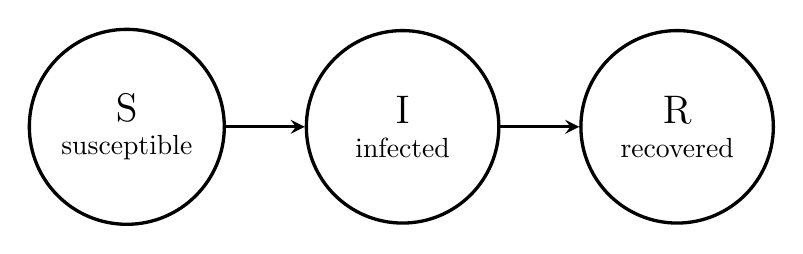
\begin{tikzpicture}[
    every node/.style={circle, draw, very thick, text width=2cm, align=center},
    every path/.style={->, >=stealth, very thick}
  ]
  \node (S) {{\Large S} \\ susceptible};
  \node (I) [right=of S] {{\Large I} \\ infected};
  \node (R) [right=of I] {{\Large R} \\ recovered};

  \draw (S) -- (I);
  \draw (I) -- (R);
\end{tikzpicture}

\end{document}
